\let\negmedspace\undefined
\let\negthickspace\undefined
\documentclass[journal,12pt,onecolumn]{IEEEtran}
\usepackage{cite}
\usepackage{amsmath,amssymb,amsfonts,amsthm}
\usepackage{algorithmic}
\usepackage{graphicx}
\usepackage{textcomp}
\usepackage{xcolor}
\usepackage{txfonts}
\usepackage{listings}
\usepackage{enumitem}
\usepackage{mathtools}
\usepackage{gensymb}
\usepackage{comment}
\usepackage{caption}
\usepackage[breaklinks=true]{hyperref}
\usepackage{tkz-euclide} 
\usepackage{listings}

\usepackage{gvv}                                        
%\def\inputGnumericTable{}                                 
\usepackage[latin1]{inputenc}     
\usepackage{xparse}
\usepackage{color}                                            
\usepackage{array}                                            
\usepackage{longtable}                                       
\usepackage{calc}                                             
\usepackage{multirow}
\usepackage{multicol}
\usepackage{hhline}                                           
\usepackage{ifthen}                                           
\usepackage{lscape}
\usepackage{tabularx}
\usepackage{array}
\usepackage{float}
%\newtheorem{theorem}{Theorem}[section]
%\newtheorem{theorem}{Theorem}[section]
%\newtheorem{problem}{Problem}
%\newtheorem{proposition}{Proposition}[section]
%\newtheorem{lemma}{Lemma}[section]
%\newtheorem{corollary}[theorem]{Corollary}
%\newtheorem{example}{Example}[section]
%\newtheorem{definition}[problem]{Definition}

\begin{document}

\title{4.4.31}
\author{AI25BTECH11035 - SUJAL RAJANI}
% \maketitle
% \newpage
% \bigskip
%\begin{document}
{\let\newpage\relax\maketitle}
%\renewcommand{\thefigure}{\theenumi}
%\renewcommand{\thetable}{\theenumi}
% \newpage
% \bigskip
\textbf{QUESTION}
\\
Find the equation of the line joining $\vec{A}$(1,3) and $\vec{B}$ (0,0).Also,find k if $\vec{D}$ (k,0) is a point such that the area of $\triangle ABD$ is 3 square units.
\\
\textbf{solution}
\\
as mentioned in the problem the position vector of the points is :
\\
\begin{align*}
    \vec{A}=\myvec{1\\3},\vec{B}=\myvec{0\\0},\vec{D}=\myvec{k\\0}
\end{align*}
the general equation of a line passing through two position vector $\vec{B}$ and $\vec{A}$ is :
\begin{align*}
    \vec{L}=\vec{H}+z\myvec{1\\m}
\end{align*}
$\vec{H}$:is either the position vector of $\vec{A}$ OR $\vec{B}$
\\
m is the slope of the line .
\begin{align*}
    m=\dfrac{y_2-y_1}{x_2-x_1}
    \\
    \vec{A}=\myvec{x_2\\y_2},\vec{B}=\myvec{x_1\\y_1}
    \\
    m=3
\end{align*}

\\
z is a constant .
\\
the equation of line passing through  $\vec{B}$ and $\vec{A}$ is :
\\
\begin{align*}
    \vec{L}=\myvec{0\\0}+z\myvec{1\\3}
\end{align*}
area of $\triangle ABD $ : 
\\
\begin{align*}
    \dfrac{1}{2}||(\vec{A}- \vec{B})X(\vec{D}- \vec{B})||=3
\end{align*}
\textbf{VECTOR PRODUCT}
\\
let N be a vector :
\begin{align}
    \vec{N}=\myvec{n_1\\n_2\\0}
    \\
    \end{align}
    let M be a vector :
    \begin{align}
    \vec{M}=\myvec{m_1\\m_2\\0}
\end{align}
the vector product of two vectors $\vec{N}$ and $\vec{M}$ is 
\\
\begin{align*}
    \vec{N}X\vec{M}=\myvec{0\\0\\n_1m_2-m_1n_2}
\end{align*}
\\
{area of $\triangle ABD$ is :}
\begin{align*}
    \dfrac{1}{2}||(\vec{A}-  \vec{B})X(\vec{D} -  \vec{B})||=\dfrac{1}{2}||\myvec{1\\3\\0}X\myvec{
    K\\0\\0}||= \dfrac{1}{2}\sqrt{\myvec{0\\0\\3K}^\top\myvec{0\\0\\3K}}=3
    \end{align*}
    \begin{align*}
        k=+2,-2
    \end{align*}
    n1=1,n2=3,m1=k,m2=0
\\

    so the position vector of $\vec{D}$ :
    \begin{align*}
        \vec{D}=\myvec{2\\0},\vec{D}=\myvec{-2\\0}
    \end{align*}

        \begin{figure}[H]
    \centering
    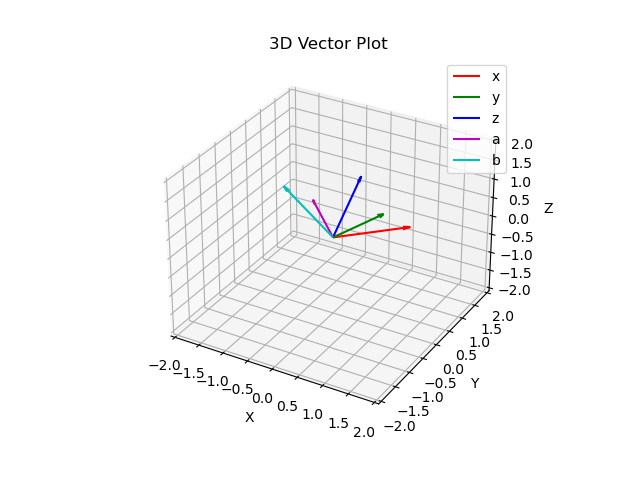
\includegraphics[width = 0.7\columnwidth]{figs/img.png}
    \caption*{}
    \label{figs}
\end{figure}

\end{document}